\documentclass[12pt,british,twoside,notitlepage,usenames,dvipsnames,hypens,final]{report}
%% Page setup
\usepackage[a4paper, twoside]{geometry}
\geometry{verbose,tmargin=3cm,bmargin=3cm,lmargin=2.5cm,rmargin=2.5cm,headheight=3cm,headsep=0.5cm,footskip=1.5cm}
\usepackage[unicode=true,
 bookmarks=true,bookmarksnumbered=true,bookmarksopen=true,bookmarksopenlevel=1,
 breaklinks=false,pdfborder={0 0 0},backref=false,colorlinks=false]
 {hyperref}
\hypersetup{pdftitle={Video Steganography using Motion Vectors -- CST Part II dissertation}, pdfauthor={E Liberis}}

\addtolength{\oddsidemargin}{6mm}
\addtolength{\evensidemargin}{-8mm}

\raggedbottom
\sloppy
\clubpenalty1000%
\widowpenalty1000%

%% Font and text flow setup
\usepackage{amsthm}
\usepackage{amsmath}
\usepackage{amssymb}
\usepackage{array}

\usepackage{polyglossia}
\setdefaultlanguage[variant=british]{english}

\usepackage{sectsty}
\allsectionsfont{\sffamily}

\usepackage{fontspec}
\setmainfont[Mapping=tex-text, Ligatures=TeX]{TeX Gyre Pagella}
\setsansfont[Mapping=tex-text, LetterSpace=1]{Gillius ADF}
\setmonofont[Mapping=tex-text]{Latin Modern Mono}

\usepackage{setspace}
\setstretch{1.1}

\setlength{\parskip}{0.5\baselineskip}
\setlength{\parindent}{0pt}

\usepackage{pifont}

%% List setup
\renewcommand\thesubsection{\arabic{subsection}.}
\usepackage{enumitem}
\setlist{nolistsep}
\setitemize{itemsep=2pt,topsep=0pt,parsep=5pt,partopsep=0pt}

%% Misc appearance things
\newtheorem{definition}{Definition}
\numberwithin{equation}{section}
\numberwithin{figure}{section}
\usepackage{multicol}
\usepackage{alltt}

\usepackage{titlesec}
\titlespacing\section{0pt}{4pt plus 0.5pt minus 0pt}{0pt plus 0.5pt minus 0.5pt}
\titlespacing\subsection{0pt}{5pt plus 4pt minus 2pt}{0.5pt plus 0.5pt minus 0.5pt}
\titlespacing\subsubsection{0pt}{5pt plus 4pt minus 2pt}{0.5pt plus 0.5pt minus 0.5pt}

\newcommand*\circled[1]{\tikz[baseline=(char.base)]{
            \node[shape=circle,draw,inner sep=2pt] (char) {#1};}}
\titleformat{\chapter}[hang]{\Huge\sf\bfseries}{\scalebox{2}{\circled{\thechapter}}}{1cm}{\Huge\bfseries}

\usepackage{epigraph}
\setlength{\epigraphrule}{0pt}

\usepackage{titletoc}
\titlecontents*{chapter}% <section-type>
  [0pt]% <left>
  {}% <above-code>
  {\sf\bfseries\chaptername\ \thecontentslabel:\quad}% <numbered-entry-format>
  {}% <numberless-entry-format>
  {\bfseries\hfill\contentspage}% <filler-page-format>

%% Some useful macros
\newcommand{\arr}{\textrightarrow\ }
\newcommand{\textsb}[1]{\textsf{\textbf{#1}}}
\newcommand{\textsbc}[1]{\sffamily \textsc{\textbf{#1}}}
\usepackage{lipsum}
\usepackage{tikz}

%%%%%%%%%%%%%%%%%%%%%%%%%%%%%%%%%%%%%%%%%%%%%%%%%%%%%%%%
\begin{document}

%% Title Page
\pagestyle{empty}

\hfill{\LARGE Edgaras Liberis}

\vspace*{60mm}
\begin{center}
\Huge
{\bf Video Steganography \\ using Motion Vectors} \\
\vspace*{10mm}
{ \sc \LARGE
Computer Science Tripos, Part II \\
Homerton College \\
}
\vspace*{10mm}
\the\year 
\end{center}

\cleardoublepage

%% Proforma
\setcounter{page}{1}
\pagenumbering{roman}
\pagestyle{plain}

{\section*{\Huge Proforma}}

{\large
\begin{tabular}{ll}
Name:               & \bf Edgaras Liberis                          \\
College:            & \bf Homerton College                         \\
Project Title:      & \bf Video Steganography using Motion Vectors \\
Examination:        & \bf Computer Science Tripos Part II, 2016    \\
Word Count:         & \bf XXXX\footnotemark[1]                     \\
Project Originator: & Edgaras Liberis                              \\
Supervisor:         & Daniel Thomas                                \\ 
\end{tabular}
}
\footnotetext[1]{This word count was computed
by {\tt detex diss.tex | tr -cd '0-9A-Za-z $\tt\backslash$n' | wc -w}
}
\stepcounter{footnote}
\vspace{0.5cm}

\section*{Original Aims of the Project}

The aim of this project is to implement and evaluate existing steganographic methods applied to motion vectors. To achieve this, an end-user tool should be developed to offer several steganographic methods. The algorithms will be evaluated based on criteria such as embedding capacity, speed, and detectability. A suite of steganalysis tools will be created.   

\section*{Work Completed}

Applications for embedding and extracting data from motion vectors were developed, featuring several popular LSB steganography algorithms. Matlab functions and scripts for steganalysis were created to extract and analyse motion vectors, offering classic and motion-vector-specific attacks against embedding schemes. Algorithms were compared against each other evaluating detectability, capacity and other aspects. Humans were used to evaluate detectability.

\section*{Special Difficulties}

None.

\cleardoublepage

%% Declaration of Originality
\section*{Declaration of Originality}
I, Edgaras Liberis of Homerton College, being a candidate for Part II of the Computer Science Tripos, hereby declare that this dissertation and the work described in it are my own work, unaided except as may be specified below, and that the dissertation does not contain material that has already been used to any substantial extent for a comparable purpose.

\bigskip
\leftline{\bf Signed }

\medskip
\leftline{\bf Date}

\cleardoublepage
\tableofcontents
%% Chapters
\renewcommand{\thesection}{\arabic{chapter}.\arabic{section}}
\renewcommand{\thesubsection}{\arabic{chapter}.\arabic{section}.\arabic{subsection}}
\setcounter{chapter}{0}

% Introduction
\cleardoublepage
\chapter{Introduction}
\pagenumbering{arabic}
\pagestyle{headings}
\setcounter{page}{1}

\emph{Steganography} is the art of concealing information within ostensibly innocent carrier data \cite[p.~3]{fridrich}, usually with the intention of creating a covert channel. Its applications include bypassing government censorship, avoiding law enforcement or military intelligence, and other situations in which detection of the communication may be harmful to the communicating parties (such as by revealing their location~\cite{infohiding-survey}). 
 
\section{Motivation}
\label{motivation}

In recent years, steganography research has explored the use of digital formats as the carrier data for hidden messages. Often, redundancy in data formats provides opportunity for concealing a payload \cite[p.~2]{fridrich}. Since multimedia formats have become so widespread online, their use is now unremarkable and unlikely to raise suspicion.

A sensible approach to digital steganography is to hide data in regions of a file that are highly tolerant to small modifications or noise, such as by slightly changing the colour of a pixel in an image. Since the least significant bit in the binary representation of a value typically corresponds to the highest granularity level, changing it is less likely to be noticed---the key concept behind the so-called \emph{least-significant-bit (LSB) embedding}~\cite{bateman}\label{lsb-steg}. 

Let us consider video steganography. The \texttt{MPEG} video format encodes a video stream as a sequence of frames. Since encoding every frame independently would be costly, the similarity of successive frames is exploited where possible to store frames as a set of changes from their predecessors. These changes are represented by how much a certain block of pixels has moved (\emph{motion vector, MV}) and how, in addition to this motion, the pixels have changed (\emph{prediction error}). Frames encoded independently are called \emph{intra-frames} or \emph{key frames} (essentially a JPEG image) and those encoded as differences called \emph{inter-frames}~\cite{h264-std}. While both hold potential as carrier data, we will be looking only at embedding data into motion vectors.

To evaluate a steganographic algorithm, we need to determine if its use is detectable by an adversary. The study of methods of detecting steganographic manipulations is called \emph{steganalysis}. Steganalysts use various domain-specific statistical attacks, such as plotting histograms, looking for correlations (or lack thereof) in the data, etc. to detect the hidden message.

This project explores hiding data in the motion vectors of \texttt{MPEG} videos by applying LSB embedding to the $x$ or $y$ components of the vector. A tool was developed to offer several high-capacity data embedding algorithms and encryption with a user-provided password. These algorithms were evaluated based on embedding capacity, speed, and detectability (using statistical steganalytic methods implemented in \texttt{Matlab}).

\section{Existing work}

Traditionally, image steganography has received more research attention than video steganography, so early attempts tried to directly use existing image (JPEG) steganography techniques~\cite{bateman, jpegdctcoding}.

Bateman reviews the evolution of LSB-based embedding algorithms~\cite{bateman}. Simple strategies such as changing the intensity of every pixel are destroyed by the lossiness of JPEG compression when the image is recompressed. This can be mitigated by embedding data into something that JPEG stores directly in a compressed file, so later research focused on using the DCT coefficients for this purpose\footnote{
One of the main compression techniques that JPEG uses is \emph{Discrete Cosine Transform (DCT)}, which is similar to the Fourier Transform. A relatively small number of coefficients is enough to reconstruct an image with sufficient quality. Those coefficients are insensitive to small changes, making they are suitable for data embedding.}~\cite{jpegdctcoding}. Other approaches improve on this by preserving statistical properties that ``clean'' images would possess~\cite{bateman, f5} (further discussed in \ref{emb-alg}). Similarly to this project, Williams~\cite{scott-fs} applies these image steganography techniques to videos by considering uncompressed videos as series of JPEG-encoded frames.

Other researchers explored inter-frame steganography using motion vectors. Xu \emph{et al.}~\cite{xu2006steganography} used the phase of an MV ($\tan^{-1}(\frac{y}{x})$) to determine which of the $x$ or $y$ component will carry a single bit of payload data (I discuss this method more in \ref{xu-alg}). Non-LSB algorithms include an interesting approach by Fang \emph{et al.}~\cite{fang2006data}, who proposed to find an alternative motion vector (with minimum prediction error), whose phase will be in a particular quadrant out of 4. This conveys 2 bits of information per MV.

One of the main deliverables of this project is a simple tool for doing MV-based steganography. Popular existing steganography tools, such as MSU StegoVideo\footnote{\url{http://www.compression.ru/video/stego_video/index_en.html}} or OpenPuff\footnote{\url{http://embeddedsw.net/OpenPuff_Steganography_Home.html}} do not implement MV steganography, so we will not discuss them further. The only implementation of MV steganography that I was able to find is James Ridgway's \emph{Steganosaurus}~\cite{steganosaurus}, but its algorithm seems rather limited. It only modifies the first (presumably the top left) motion vector of every frame, severely limiting embedding capacity and increasing the ease of detection (as the location of the modified MV is known).

Meanwhile, steganalysis exploited properties specific to motion vectors to create novel steganalysis methods. A recurrent approach in these methods is developing a system to extract certain statistical features from videos and use them to train a classifier. Xu \emph{et al.}~\cite{xu2013video} proposed to build a set of vector algebra constraints between MVs across several frames for this purpose. Deng \emph{el al.}~\cite{deng2012digital} observes that neighbouring MVs often have the same motion vectors, so an abnormal MV can be spotted. Surprisingly, Cao \emph{et al.}~\cite{cao2012video} argues that simply transcoding\footnote{Unpacking a video into a sequence of images and recompressing it back again.} a video would revert a significant amount of MVs to their original values. This reversion technique is evaluated in \ref{rev-tech}.

\subsection*{Outline of the rest of the document}
\textbf{TODO}
\begin{itemize}
\item Chapter 2 (Preparation) discusses relevant theoretical background on steganography, steganalysis and video encoding in more detail, and justifies the use of motion vectors as an embedding space. This is followed by the development plan, which decides on deliverables and their formal requirements, existing tools and libraries that the project builds upon, technical choices, theoretical starting point and software engineering approaches employed.
\item Chapter 3 (Implementation) describes implementation specifics for the steganographic tool, steganalysis package and embedding algorithms, with some in-line evaluation of detectability.
\item Chapter 4 (Evaluation) discusses remaining aspects of evaluation, such as speed, capacity, automatic classification and experiment on human subjects.
\item Chapter 5 (Conclusions) summarises the work done, describes successes and shortcomings of the project and gives ideas for potential improvements.
\end{itemize}
 

% Preparation
\cleardoublepage
\chapter{Preparation}

\textit{This chapter presents the theory behind steganography and steganalysis in more detail, covers relevant video encoding principles and makes an argument in favour of using motion vectors for video steganography. This is followed by a discussion about project's software deliverables, formal requirements, existing libraries and tools leveraged, risk analysis, workflow and starting point. } 

\section{Steganography Background}

This project is concerned with the development of a \emph{steganographic system}, so let us review terminology used in the field~\cite{infohiding-survey, bateman}:
\begin{itemize}
\item \emph{Embedded data / payload} --- the message that one wishes to hide.
\item \emph{Carrier / carrier data / cover-object / cover-video / cover} --- an object (video) that will contain the embedded data.
\item \emph{Stego-object / stego-video / container } --- an object (video) that contains the embedded data.
\item \emph{Stego-key} ---  data that is used to ``control the embedding process and/or to restrict detection and/or recovery of the embedded data to parties who know it"~\cite{infohiding-survey}. This could be a user-provided password which is later used to seed a PRNG\footnote{Pseudo Random Number Generator} or derive encryption keys. 
\item \emph{Embedding space} --- a particular type or region of data in a cover-object that is suitable for carrying the payload, e.g. DCT coefficients in JPEG.
\item \emph{Embedding capacity} --- the amount of information (in bits) a particular embedding scheme can hide within a certain cover. Typically it also depends on the payload as well, but we relax this condition for now.
\item \emph{Covert communication} -- communication performed by sending stego-objects. 
\end{itemize}

A more formal definition of a steganographic system~\cite{scott-fs}, that manipulates the cover to embed the data is as follows:

\begin{definition}{Steganographic System}

Let $\mathcal{C}$ be the set of all cover objects. For a given $c \in C$, let $\mathcal{K}_c$ denote the set of all stego keys for $c$, and the set $\mathcal{M}_c$ denote all messages that can be communicated in c. A steganographic system is then formally defined as a pair of embedding and extracting functions \texttt{Emb} and \texttt{Ext},
\begin{align*}
\texttt{Emb} &: \mathcal{C} \times \mathcal{K} \times \mathcal{M} \rightarrow \mathcal{C} \\
\texttt{Ext} &: \mathcal{C} \times \mathcal{K} \rightarrow \mathcal{M}
\end{align*}
such that
\begin{align*}
\forall c \in \mathcal{C}, k \in \mathcal{K}_c, m \in \mathcal{M}_c . ~ \texttt{Ext}(\texttt{Emb}(c, k, m), k) = m
\end{align*}

\end{definition}

In other words, a steganographic system (also referred to as \emph{embedding scheme / algorithm / method}) is defined by providing \emph{embedding} (encoding) and \emph{extracting} (decoding) functions, which describe how payload's bits should be embedded within (or extracted from) the cover.

A steganographic system aims to protect the embedded data from being detected by an adversary. Therefore we should make some reasonable assumptions about adversary's capabilities prior to discussing system's security properties. Steganography considers three types of adversaries~\cite{craver1998public}:
\begin{itemize}
\item \emph{Passive warden} -- an adversary who can only spy on the communication.
\item \emph{Active warden} -- an adversary who can perform reasonable modifications to the stego-object (e.g. by cropping the stego-image).
\item \emph{Malicious warden} -- an adversary who can significantly modify the payload or try to impersonate either party.
\end{itemize}
Warden analogy comes from thinking about communicating parties as if they were communicating prisoners and the warden is passing messages between cells~\cite{craver1998public}. 
This project is only concerned with passive wardens, stego-videos are not expected to withstand resizing, transcoding, \emph{etc.}

A steganographic system that relies on so-called `security through obscurity' is generally frowned upon, as it is just a matter of time before an adversary figures out how the system works. This is addressed by \emph{Kerckhoffs' principle} (first formulated for cryptographic systems), which states that one should assume that the system is known to the enemy, so ``security must lie only in the choice of key"~\cite{infohiding-survey}. In steganographic systems that is achieved by introducing a \emph{stego-key} which is assumed to be already known to all parties. Schemes implemented in the project use it for two purposes:

\begin{itemize}
\item If the embedding space of a cover-object has \emph{random noise}, schemes can hide the payload within it. This requires the payload to be indistinguishable from the random noise which is achieved by encrypting it. Encryption key can be derived from the stego-key.

\item Consider a scheme that spreads the payload over the cover, e.g. by selecting a location for each bit of the payload at random. This requires both parties to have a synchronised PRNG\footnote{PRNGs are synchronised if they generate an identical sequence of pseudo-random numbers.}, which can be achieved by seeding a known generator with the same seed --- the stego-key.
\end{itemize}
\section{Steganalysis Background}

Steganalysis is the study of detecting messages produced by steganographic systems~\cite[p.~10]{fridrich}. A steganographic system is considered broken if a steganalyst, given an object, is able to tell whether it contains the hidden payload with a probability better than a random guess.

The most trivial example of steganalysis is when an adversary is given an original cover-object together with the ostensibly-stego-object. Then telling whether the latter actually contains the payload is just a matter of comparing the two. 

Steganalytic techniques can be either manual or automated, and can be further split into two broad categories~\cite{bateman}:
\begin{itemize}
\item \emph{Targeted Steganalysis.} Steganalyst looks for abnormalities and traces left by a known embedding scheme using visual or statistical attacks specific to a particular scheme.
\item \emph{Blind Steganalysis.} Steganalyst doesn't assume a particular scheme and instead looks whether properties of the given object match those normally expected from that kind of objects. 
\end{itemize} 

This project implements both targeted and blind steganalysis methods against motion vector steganography.

\section{Video Steganography}

The project uses MPEG video files as containers for embedded data. We explore the MPEG format in more detail to see whether motion vectors is a feasible embedding space in terms of detectability and embedding capacity.  

\subsection{Video encoding background}

A video \emph{codec} (en\underline{co}der + \underline{dec}oder) is an application that takes a series of images (video frames) and compresses it into a single video file or vice versa \cite[sec.~3.1]{richardson2004h}. MPEG (Moving Picture Experts Group) family of codecs is the most common choice for video compression.

As discussed in \ref{motivation}, MPEG video stream is represented by a series of interleaved \emph{intra-} and \emph{inter-frames}. Intra-frames are also known as \emph{I-frames} and inter-frames are further classified into \emph{P-frames} or \emph{B-frames}. P- (prediction) frames encode an image by only looking at the predecessor frame, whereas B- (bidirectional) frames consider both predecessor and successor frames [Fig.~\ref{fig:ipb-seq}]~\cite{crowcroft1999internetworking}. To simplify the implementation, from now on I will only consider P-frames, although, in principle, all methods should apply equally well to B-frames too.

\begin{figure}[tbh]
\centerline{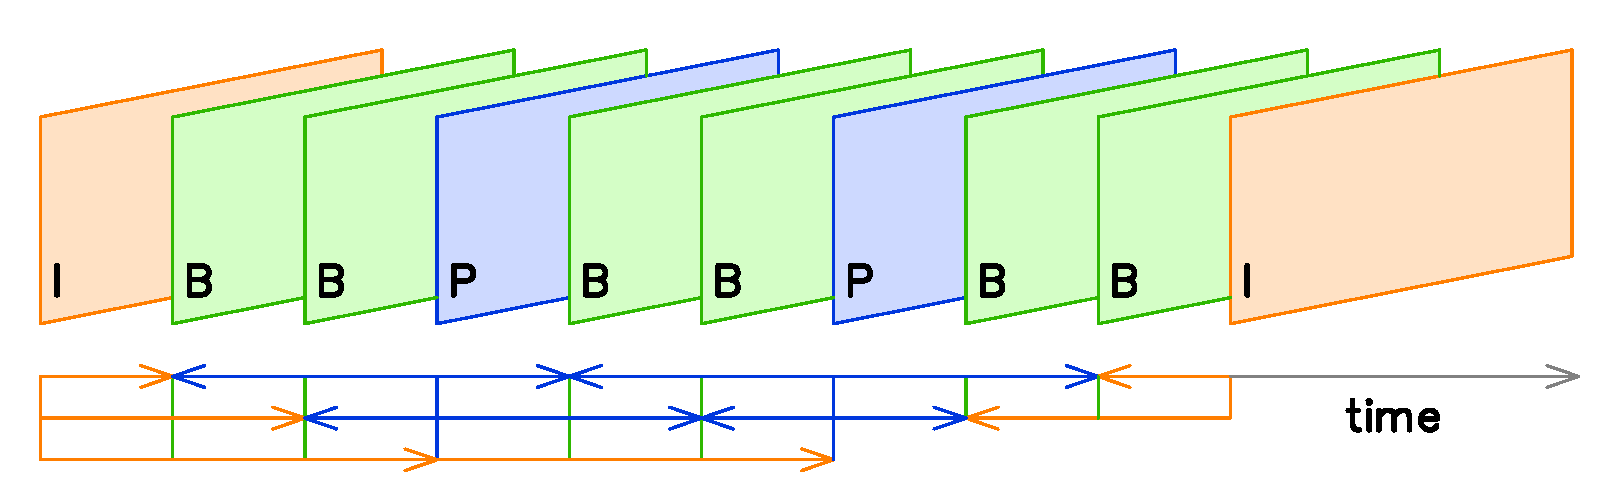
\includegraphics[width=0.7\textwidth, height=0.7\textheight, keepaspectratio]{img/IPB_images_sequence.png}}
\caption{An example of interleaved I-, B- and P-frames representing a video stream. The encoder may choose a different sequence of frame types. Reproduced from~\cite{interframe-wiki}.}
\label{fig:ipb-seq}
\end{figure}

During the encoding, a frame which will be encoded as a P-frame is partitioned into a grid of blocks of size 16-by-16 pixels\footnote{H.264 allows higher granularity for fine details by allowing some blocks to be 8x8, 8x16 or 16x8.}. These blocks are called \emph{macroblocks}, and for each macroblock the encoder searches for its most similar match in a predecessor frame within a bounded search window \cite[p.~256]{richardson2004h}. The difference of pixels between the match and the original block is called \emph{prediction error}, and the position difference of the two is called \emph{motion vector} [Fig.~\ref{fig:mb-search}]. For simplicity, we say that a block of pixels has moved since the predecessor frame by the amount specified by its motion vector and, in addition to motion, pixels themselves have changed according to the prediction error.

\begin{figure}[tbh]
\centerline{\includegraphics[width=0.7\textwidth,height=0.7\textheight,keepaspectratio]
{img/macroblock-diagram.png}}
\caption{An illustration of a macroblock search from the current (target) frame to the predecessor (reference) frame. A macroblock is encoded using its prediction error and  motion vector.}
\label{fig:mb-search}
\end{figure} 

\subsection{Motion vectors as embedding space}

Computing motion vectors is a tradeoff between accuracy and computation time, adjusted by the search window size. Therefore codecs typically settle for an approximation instead of an optimal MV, resulting in a non-minimal prediction error \cite[p.~257]{richardson2004h}. While MVs are encoded losslessly, this accuracy tradeoff allows minor changes to them go unnoticed: a property that makes them suitable for LSB steganography (see \ref{lsb-steg}).

To estimate the embedding capacity, let us generalise how all implemented embedding schemes should operate on motion vectors. Suppose an embedding scheme processes every motion vector in a grid individually for every frame, and has an associated selection function $f$, which provides a number of bits that can be embedded into that motion vector ($f(\overrightarrow{mv}) = 0$, if an MV is unused). Later on, this will allow to conveniently define a MV selection criteria for different embedding schemes.

\begin{definition}{Embedding capacity for video}

Let $M$ be an embedding scheme with an associated function $f_M : \mathbb{R}^2 \rightarrow \mathbb{N}$, which calculates how many bits can be embedded into a particular motion vector $\overrightarrow{mv} \in \mathbb{R}^2$. Then for an MPEG-encoded video $V$, the embedding capacity $\mathcal{C}_{V, M}$ is defined as:

$$ \mathcal{C}_{V, M} = \sum_{p \in \text{P-frames}(V)} \: \sum^{H}_{j = 0} \sum^{W}_{i = 0} f_M(\overrightarrow{mv}^p_{i, j})$$

where $W$ and $H$ are width and height of the macroblock grid, P-frames$(V)$ is a set of all P-frames of a video $V$ and $\overrightarrow{mv}^p_{i, j}$ is the MV of a macroblock  in $i$-th row and $j$-th column of the frame $p$.

\end{definition}

To see that videos could generally hold a non-negligible amount of hidden data, we can estimate $\mathcal{C}_{V, M}$ by taking a product of the number of P-frames, the total number of MVs per frame and the average number of bits embedded per MV. An average HD video could reasonably have 6--15 P-frames per second\footnote{Depends on how often the encoder decides to use B-frames and I-frames. P-frames are better for video streaming as they do not require the successor frame to be known during decoding.} with 3600 MVs each\footnote{If video's resolution is 1280x720 (HD), 16x16 macroblocks would partition the frame into a grid of size 80x45. This gives 3600 macroblocks in total.}. Assuming only a quarter of each frame would contain hidden data, we estimate the channel's capacity to be 5.4--13 Kbits/s, which is higher than for any other popular digital media format.

\section{Requirements analysis}

The project consists of two main software deliverables:
\begin{itemize}
\item  An application that allows the user to embed secret messages into MPEG video files using a selection of LSB embedding algorithms.
\item A steganalysis suite that implements some general-purpose routines to detect motion vector-based steganography.
\end{itemize}

Below is a list of requirements for both deliverables, prioritised using \emph{MoSCoW} model.

\subsection{Steganographic Application}
\begin{itemize}
\item (M) Ability to access motion vectors of an MPEG video file.
\item (M) Ability to reliably embed data within motion vectors.
\item (M) Multiple LSB embedding techniques.
\item (M) User-friendly binaries to perform embedding and extraction.
\item (S) Encryption of the secret message prior to embedding.
\item (S) Integration with an existing video codec.
\end{itemize}

\subsection{Steganalysis Suite}
\begin{itemize}
\item (M) Ability to extract and process motion vector data.
\item (M) Multiple steganalysis methods.
\item (M) Documentation on usage and interpretation of the results.
\item (M) Evident effectiveness in detecting implemented embedding techniques.
\item (S) Compatibility with existing scientific computation packages (Matlab or Python-based packages)
\item (S) Usefulness (verbosity, amount of information provided) to the steganalyst.
\end{itemize}

\section{Project workflow}

\subsection{Technical choices}

Steganographic application requires modifying MPEG video files, which in turn requires parsing the format of a file, modifying motion vector values, and repackaging the data back into a valid playable video. Developing a codec does not relate to steganography and is potentially error prone, so I leverage an existing set of codecs---\texttt{FFmpeg}\footnote{\url{https://www.ffmpeg.org/}}---to achieve this. As codecs are typically written in C or C++, it is a natural choice for this task to and makes the integration easier.

Performing encryption prior to embedding requires using a cryptography library. \emph{Crypto++}, a popular C++ cryptography implementation, is used in the project.

Steganalysis suite was integrated into a scientific computation package, because it provides useful tools, such as statistical primitives, plotting capabilities, classifiers, \textit{etc.} without changing the environment, which benefits the user. The choice was made in favour of Matlab due to its widespread use and comprehensive functionality.

\subsection{Risk analysis}
FFmpeg is a complex piece of software, mostly written in a style of C that sacrifices clarity for performance. A potential risk for the project was the difficulty of proper integration with FFmpeg and hence inability to access or reliably modify motion vectors. Complete failure to do so was very unlikely, but nevertheless it could have consumed a significant amount of development time. To mitigate this, some ``catch-up'' time was allocated in the project timetable.  

\subsection{Workflow}
\begin{itemize}
\item \emph{Git} was used for version control, allowing quick roll-back and managing multiple source trees using branches.
\item \emph{Backups} were done by uploading the source tree and other relevant files to Dropbox. The git repository itself was hosted remotely on GitHub.
\item \emph{Testing} \textbf{TODO}
\item \emph{Interative (spiral) development model} was used continuously add and test new embedding techniques and steganalysis methods to the project.
\end{itemize}

\section{Starting Point}
This project uses some cryptography concepts introduced in the Part IB \textit{Security I} course. I have had some C++ knowledge from past programming experience and the \textit{Programming in C and C++} course. 

Prior to submitting the proposal, I have familiarised myself with the general concepts of steganography and LSB embedding though some introductory texts and relevant papers, and briefly looked at H.264 codec format.

During the development of this project I made use of some material covered in the following Part II courses:
\begin{itemize}
\item \textit{Information Theory} --- channel capacity, error correcting codes,
\item \textit{\LaTeX~and Matlab} --- typesetting and basics of Matlab,
\item \textit{Artificial Intelligence II} --- classifier evaluation.
\end{itemize}

\bigskip
This chapter summarised relevant theoretical and practical background necessary to start the implementation. Next chapter will cover the design and features of the system, implemented steganographic algorithms and steganalysis methods, with some in-line evaluation.

% Implementation
\cleardoublepage
\chapter{Implementation}

Coherent summary of the following chapter, quickly outlining approach taken.

\section{Embedding and decoding process}

\subsection{Encoder}

How is encoder implemented? Structure, schematic, interesting parts.  Frame independence assumption.

\subsection{Decoder}

How is decoder implemented? Structure, schematic, interesting parts. 

\section{Steganalysis techniques}

\subsection{Functions Supporting Extraction}

Typed / untyped MVs; sequential decoder

\subsection{LSB Plane + PLOT}

\subsection{Histogram}

\subsection{$\chi^2$ (Chi-Squared) Attack}

In general terms, don't tailor to MV case very much yet.

\subsection{Reversion Technique}
Implementation of data processor and SVM.

\section{Embedding algorithms}
\label{emb-alg}

\subsection{Hide and Seek}

What's it about, outline basic concepts. Show histogram detectability.

\subsection{MSteg}

Why it avoids 0 and 1. Histogram motivation. Show equal pairs.

\subsection{F3}

Shirinkage. Effects of that. Histogram attack.

\subsection{F4}

How it avoids histogram attack? Chi-square attack on sequential attack.

\subsection{Randomised Hide-n-Seek}

Explain upsides of randomised embedding. Impl issues, mention ECC. 

\subsection{Outguess 0.1}

Similarly avoids 0s and 1s as most detectable ones. Current attack is JPEG specific?

\subsection{Xu's Algorithm}
\label{xu-alg}

Discuss how MVSteg should be implemented + design decisions.

\section{Application}

\subsection{Design \& Usage}

Discuss implementation \& integration with libraries done.

\subsection{Encryption}
Discuss encryption features of the application.

\subsection{Initially proposed extensions}
Comment on why it didn't work out.

%**F5????**
%Minimising number of changes made to MVs

\section{Testing}

Discuss testing, manual / automatic.

% Evaluation
\cleardoublepage
\chapter{Evaluation}

Coherent summary of the following chapter, quickly outlining evaluation approaches.

\section{Evaluation of embedding and decoding process}

Say / evaluate what was done for embedding / decoding modules. Anything interesting? Difficulties encountered? Does app do what is expected, usability?

\section{Evaluation of embedding algorithms}

\subsection{Fixing Xu's algorithm}

Dubious thresholding on length, see histograms. Which way to go?
Detectable angle thresholding.
Detectable embedding 4x.
Potential attack using the reversion technique (and mention tools again here).

\subsection{Reversion Technique}
\label{rev-tech}

What is the result on the dataset per algorithm?

\subsection{Embedding capacity}

Talk about the differences (esp. randomised).

\subsection{Speed}

Mention how fast transcoding is

\subsection{Detectability by Humans (Study)}

\subsubsection{Hypothesis}

\subsubsection{Experimental procedure}

\subsubsection{Results}

Was the study hypothesis confirmed?

% Conclusions
\cleardoublepage
\chapter{Conclusions}

Say that project was a success.

\section{Summary}

\section{Lessons learnt}

\section{Future directions}

People suggest different approaches, mention some. Is it really white noise?

\cleardoublepage
\bibliographystyle{unsrt}
\bibliography{refs}

\end{document}